\section{Versuchsaufbau}
In diesem Versuch wird ein koaxialer Germanium-Detektor verwendet,
dessen Oberfläche durch einen Metall-Halbleiterkontakt mit Lithium charakterisiert ist. Das heißt, es handelt 
sich um eine Zylinder mit einem Durchmesser von $\SI{45}{\milli\meter}$ und einer 
Länge von $\SI{39}{\milli\meter}$. 
Im Inneren des Detektors wurde eine koaxiale Bohrung vorgenommen und mit Gold 
bedampft, um eine Verarmungszone zu erzeugen. 
Über dem Detektor befindet sich eine Aluminumkappe, die die Gammastrahlung dazu zwingt, 
durch sie und durch die dotierte Lithiumoberfläche hindurch zu dringen, um detektiert zu werden.
Diese Kappe schützt den Lithium-Germanium-Kontakt vor Verunreinigungen und verkleinert 
effektiv das zu kühlende Volumen.
Dadurch kommt es zu einer unteren Energienachweisgrenze bei 
$\SI{40}{\kilo\electronvolt}$ bis $\SI{50}{\kilo\electronvolt}$.
Um eine volle Energeinachweiswahrscheinlichkeit zu erhalten, sollten  Energien über 
$\SI{150}{\kilo\electronvolt}$ verwendet werden. 
Der Aufbau ist in Abbildung \ref{abb1} graphisch dargestellt \cite{sample}.

\begin{figure}
    \centering
    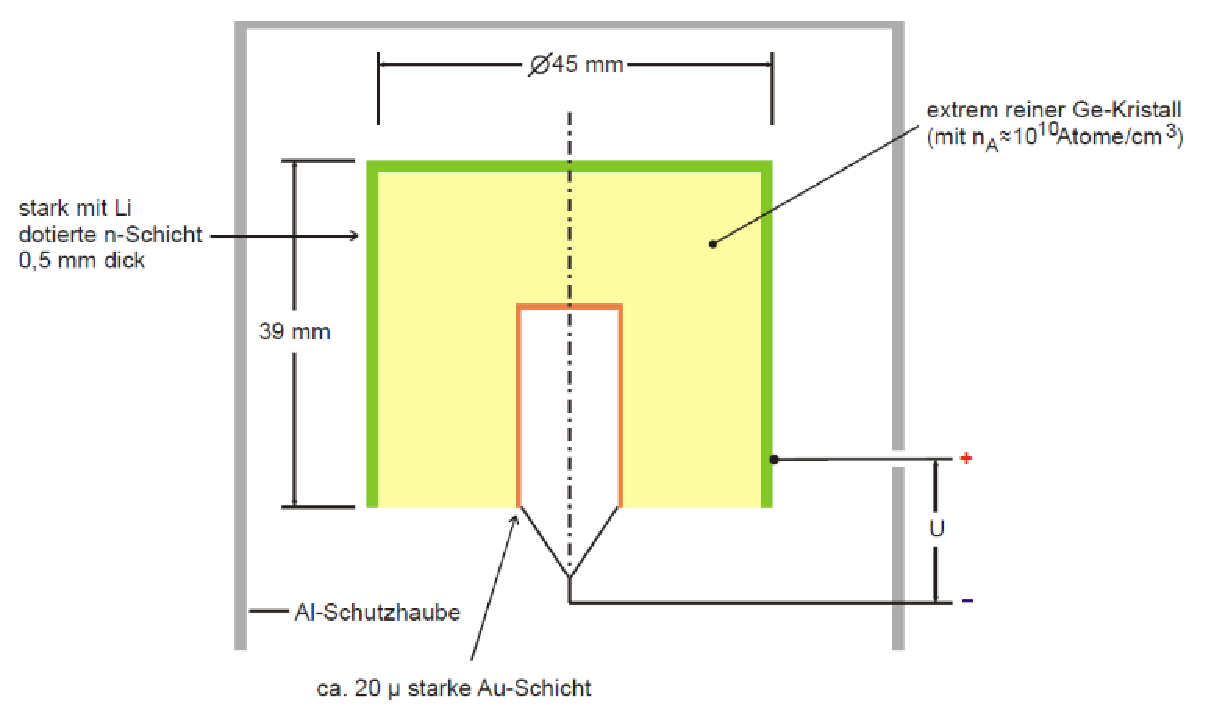
\includegraphics[width=\textwidth]{figure/Aufbau.pdf}
    \caption{Diese Abbildung veranschaulicht den Versuchsaufbau des Halbleiter-Germamium-Detektors \cite{sample}.}
    \label{abb1}
\end{figure}



\section{Durchführung}
\label{sec:Durchführung}

In diesem Versuch werden vier Messreihen durchgeführt. 
Zunächst soll eine Energiekalibrierung der Apparatur vorgenommen werden und eine 
Messung der Vollenergienachweiswahrscheinlichkeit durchgeführt werden.
Dafür wird das Spektrum eines \ce{^152Eu}-Strahlers aufgenommen, sodass die Lage 
als auch der Inhalt der Linien bestimmt werden kann.
Danach wird das Spektrum eines \ce{^137Cs}-Strahlers aufgenommen, um den Photoeffekt 
und die Compton-Streuung zu vergleichen.
Eine der Strahungsquellen \ce{^125Sb} und \ce{^133Ba} wird vermessen und anhand ihres 
Spektrums wird sie identifiziert. Außerdem wird die Aktivität der Quelle
bestimmmt.
Als letztes wird ein Anwendungsfall durchgespielt. 
Es wird das Spektrum eines unbekannten Strahlers aufgenommen und  
seine Zusammensetzung bestimmt \cite{sample}.
